% v6.0 Pairwise Model Correlation Heatmap
% Replaces: tab:error-correlations in appendix_m
% Manual heatmap showing prediction error correlations between ensemble components

\begin{figure}[htbp]
\centering
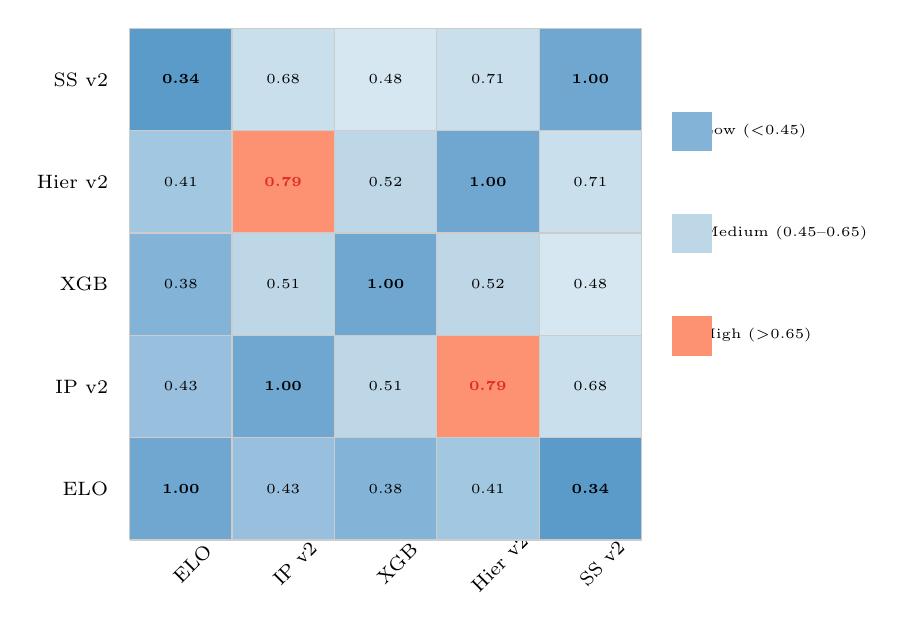
\begin{tikzpicture}
% Define correlation-to-color mapping
\definecolor{lowcorr}{RGB}{49,130,189}
\definecolor{midcorr}{RGB}{189,215,231}
\definecolor{highcorr}{RGB}{252,146,114}
\definecolor{vhighcorr}{RGB}{222,45,38}

% Cell size
\def\cellsize{1.3}

% Row/column labels
\foreach \name/\y in {ELO/0, IP v2/1, XGB/2, Hier v2/3, SS v2/4} {
  \node[font=\scriptsize, anchor=east] at (-0.15, \y*\cellsize+\cellsize/2) {\name};
  \node[font=\scriptsize, anchor=north, rotate=45] at (\y*\cellsize+\cellsize/2, -0.15) {\name};
}

% Helper: draw cell with color and text
% Data matrix (lower triangle + diagonal):
% SS-SS=1.00 SS-Hier=0.71 SS-XGB=0.48 SS-IP=0.68 SS-ELO=0.34
% Hier-Hier=1.00 Hier-XGB=0.52 Hier-IP=0.79 Hier-ELO=0.41
% XGB-XGB=1.00 XGB-IP=0.51 XGB-ELO=0.38
% IP-IP=1.00 IP-ELO=0.43
% ELO-ELO=1.00

% Row 0 (ELO): ELO-ELO, ELO-IP, ELO-XGB, ELO-Hier, ELO-SS
\fill[lowcorr!70] (0,0) rectangle +(\cellsize,\cellsize);
\fill[lowcorr!50] (\cellsize,0) rectangle +(\cellsize,\cellsize);
\fill[lowcorr!60] (2*\cellsize,0) rectangle +(\cellsize,\cellsize);
\fill[lowcorr!45] (3*\cellsize,0) rectangle +(\cellsize,\cellsize);
\fill[lowcorr!80] (4*\cellsize,0) rectangle +(\cellsize,\cellsize);

% Row 1 (IP): IP-ELO, IP-IP, IP-XGB, IP-Hier, IP-SS
\fill[lowcorr!50] (0,\cellsize) rectangle +(\cellsize,\cellsize);
\fill[lowcorr!70] (\cellsize,\cellsize) rectangle +(\cellsize,\cellsize);
\fill[midcorr] (2*\cellsize,\cellsize) rectangle +(\cellsize,\cellsize);
\fill[highcorr] (3*\cellsize,\cellsize) rectangle +(\cellsize,\cellsize);
\fill[midcorr!80] (4*\cellsize,\cellsize) rectangle +(\cellsize,\cellsize);

% Row 2 (XGB): XGB-ELO, XGB-IP, XGB-XGB, XGB-Hier, XGB-SS
\fill[lowcorr!60] (0,2*\cellsize) rectangle +(\cellsize,\cellsize);
\fill[midcorr] (\cellsize,2*\cellsize) rectangle +(\cellsize,\cellsize);
\fill[lowcorr!70] (2*\cellsize,2*\cellsize) rectangle +(\cellsize,\cellsize);
\fill[midcorr] (3*\cellsize,2*\cellsize) rectangle +(\cellsize,\cellsize);
\fill[midcorr!60] (4*\cellsize,2*\cellsize) rectangle +(\cellsize,\cellsize);

% Row 3 (Hier): Hier-ELO, Hier-IP, Hier-XGB, Hier-Hier, Hier-SS
\fill[lowcorr!45] (0,3*\cellsize) rectangle +(\cellsize,\cellsize);
\fill[highcorr] (\cellsize,3*\cellsize) rectangle +(\cellsize,\cellsize);
\fill[midcorr] (2*\cellsize,3*\cellsize) rectangle +(\cellsize,\cellsize);
\fill[lowcorr!70] (3*\cellsize,3*\cellsize) rectangle +(\cellsize,\cellsize);
\fill[midcorr!80] (4*\cellsize,3*\cellsize) rectangle +(\cellsize,\cellsize);

% Row 4 (SS): SS-ELO, SS-IP, SS-XGB, SS-Hier, SS-SS
\fill[lowcorr!80] (0,4*\cellsize) rectangle +(\cellsize,\cellsize);
\fill[midcorr!80] (\cellsize,4*\cellsize) rectangle +(\cellsize,\cellsize);
\fill[midcorr!60] (2*\cellsize,4*\cellsize) rectangle +(\cellsize,\cellsize);
\fill[midcorr!80] (3*\cellsize,4*\cellsize) rectangle +(\cellsize,\cellsize);
\fill[lowcorr!70] (4*\cellsize,4*\cellsize) rectangle +(\cellsize,\cellsize);

% Grid lines
\foreach \i in {0,...,5} {
  \draw[gray!40] (\i*\cellsize, 0) -- (\i*\cellsize, 5*\cellsize);
  \draw[gray!40] (0, \i*\cellsize) -- (5*\cellsize, \i*\cellsize);
}

% Text labels in cells
\node[font=\tiny\bfseries] at (0.5*\cellsize, 0.5*\cellsize) {1.00};
\node[font=\tiny] at (1.5*\cellsize, 0.5*\cellsize) {0.43};
\node[font=\tiny] at (2.5*\cellsize, 0.5*\cellsize) {0.38};
\node[font=\tiny] at (3.5*\cellsize, 0.5*\cellsize) {0.41};
\node[font=\tiny\bfseries] at (4.5*\cellsize, 0.5*\cellsize) {0.34};

\node[font=\tiny] at (0.5*\cellsize, 1.5*\cellsize) {0.43};
\node[font=\tiny\bfseries] at (1.5*\cellsize, 1.5*\cellsize) {1.00};
\node[font=\tiny] at (2.5*\cellsize, 1.5*\cellsize) {0.51};
\node[font=\tiny\bfseries, text=vhighcorr] at (3.5*\cellsize, 1.5*\cellsize) {0.79};
\node[font=\tiny] at (4.5*\cellsize, 1.5*\cellsize) {0.68};

\node[font=\tiny] at (0.5*\cellsize, 2.5*\cellsize) {0.38};
\node[font=\tiny] at (1.5*\cellsize, 2.5*\cellsize) {0.51};
\node[font=\tiny\bfseries] at (2.5*\cellsize, 2.5*\cellsize) {1.00};
\node[font=\tiny] at (3.5*\cellsize, 2.5*\cellsize) {0.52};
\node[font=\tiny] at (4.5*\cellsize, 2.5*\cellsize) {0.48};

\node[font=\tiny] at (0.5*\cellsize, 3.5*\cellsize) {0.41};
\node[font=\tiny\bfseries, text=vhighcorr] at (1.5*\cellsize, 3.5*\cellsize) {0.79};
\node[font=\tiny] at (2.5*\cellsize, 3.5*\cellsize) {0.52};
\node[font=\tiny\bfseries] at (3.5*\cellsize, 3.5*\cellsize) {1.00};
\node[font=\tiny] at (4.5*\cellsize, 3.5*\cellsize) {0.71};

\node[font=\tiny\bfseries] at (0.5*\cellsize, 4.5*\cellsize) {0.34};
\node[font=\tiny] at (1.5*\cellsize, 4.5*\cellsize) {0.68};
\node[font=\tiny] at (2.5*\cellsize, 4.5*\cellsize) {0.48};
\node[font=\tiny] at (3.5*\cellsize, 4.5*\cellsize) {0.71};
\node[font=\tiny\bfseries] at (4.5*\cellsize, 4.5*\cellsize) {1.00};

% Legend
\node[font=\tiny, anchor=west] at (5.5*\cellsize, 4*\cellsize) {Low ($<$0.45)};
\fill[lowcorr!60] (5.3*\cellsize, 3.8*\cellsize) rectangle +(0.5,0.5);
\node[font=\tiny, anchor=west] at (5.5*\cellsize, 3*\cellsize) {Medium (0.45--0.65)};
\fill[midcorr] (5.3*\cellsize, 2.8*\cellsize) rectangle +(0.5,0.5);
\node[font=\tiny, anchor=west] at (5.5*\cellsize, 2*\cellsize) {High ($>$0.65)};
\fill[highcorr] (5.3*\cellsize, 1.8*\cellsize) rectangle +(0.5,0.5);

\end{tikzpicture}
\caption[Error correlation heatmap]{Pairwise prediction error correlations (v6.0 ensemble, 2022--2024). ELO exhibits lowest correlations (0.34--0.43, blue), providing maximum diversification despite smallest weight. Hierarchical--Informative Priors pair shows highest correlation (0.79, red), reflecting shared Bayesian foundations. Low off-diagonal correlations confirm ensemble diversity.}
\label{fig:error-correlations-chart}
\end{figure}
